\chapter{Intellectual Property and Non-Competes}\label{ch:fm:intellectual-property-and-non-competes}

On 5 June 2009, his last day at Goldman Sachs, a programmer who had worked on the bank's high-frequency trading system encrypted and uploaded
more than 500\,000 lines of its source code to a server in Germany; he had accepted a job at a start-up building its own trading system. A jury
convicted him under two federal statutes and he was sentenced to 97 months in prison. In 2012 the Court of Appeals for the Second Circuit reversed
both convictions: the code, it held, was not a stolen ``good'' under one statute, and under the other it was not related to a product ``produced
for or placed in interstate or foreign commerce'', since the bank sold and licensed its trading system to no one. Within the year Congress
amended the second statute to cover products and services used in commerce. A trading firm's most valuable assets are written in code and
carried in people's heads, and the law that protects them turns on words like these.

\section{What a trading firm owns: code, models, data and know-how}

A trading firm's capital, premises and connections can be bought. What it owns that a competitor cannot buy is a set of things that are hard to see
and easy to carry: source code, the structure of its models and their fitted parameters, cleaned and joined data, research logs (One Quant Book 7)
recording what was tried and what failed, and the know-how of the people who built them. Most of it is protected in only two ways. Either the law
treats it as a secret and punishes its taking, or contracts keep the people who know it from using it elsewhere for a while.

Patents and copyright do little of the work. A trading strategy is rarely patentable, and patenting it would publish it; copyright protects the
text of code but not the idea it implements, and a competitor who rewrites a model from memory copies no text. So the firm's protection rests on
secrecy, and secrecy is a matter of degree: every departure, every conference talk and every vendor who sees the data leaks some of it.

Three things differ in how fast what leaks loses its value.
\begin{itemize}
\item \textbf{The model's structure}: which effects the strategy trades and how it combines them. It decays slowly, at the pace of the effect
itself: crowding and post-publication decay (One Quant Book 7) erode it over years.
\item \textbf{The parameters}: the fitted weights, thresholds and sizes. Their value is high but short: they are re-fitted every few months, and a
stale copy loses its edge quickly.
\item \textbf{The data}: the pipeline that cleans and joins the inputs. Its value decays at the pace of the vendors' own changes.
\end{itemize}
The chapter's model gives each a share of the strategy's profits that a competitor using it would take, and a half-life, the time for the value of
what was taken to halve, which is Book 7's signal half-life applied to the leaked knowledge.

\section{Trade secrets and how they are protected}

\begin{definition}[Trade secret]\label{def:fm:intellectual-property-and-non-competes:secret}
A \emph{trade secret}\index{trade secret} is information, including source code, models and data, that is not generally known or readily
ascertainable by others in the field, that has commercial value because it is secret, and that its holder has taken reasonable steps to keep
secret.
\end{definition}

The three conditions are nearly the same in the United States, the European Union and the United Kingdom (\cref{dat:fm:intellectual-property-and-non-competes:law}).
The third is the one a firm controls, and the one litigation turns on: a court asks what the firm did, not what it intended. The reasonable steps
are ordinary controls: access on a need-to-know basis, logging of copies and uploads, segregation of duties (One Quant Book 6) between those who
write code and those who can move it off the firm's systems, and contracts.

\begin{definition}[Confidentiality agreement, invention assignment clause]\label{def:fm:intellectual-property-and-non-competes:nda}
A \emph{confidentiality agreement}\index{confidentiality agreement} binds an employee or counterparty not to disclose or use the firm's
confidential information, during and after the relationship. An \emph{invention assignment clause}\index{invention assignment clause} in an
employment contract assigns to the employer the rights in work the employee creates in the course of the employment: code, models, research and
documents.
\end{definition}

\begin{dated}{2026-09}{Trade secret law}\label{dat:fm:intellectual-property-and-non-competes:law}
\textbf{United States}: 18 U.S.C. 1839(3) defines a \omterm{def:fm:intellectual-property-and-non-competes:secret}{trade secret} as financial, business, scientific, technical, economic or engineering
information, including programs and codes, whose owner has taken reasonable measures to keep it secret and which derives independent economic
value from not being generally known or readily ascertainable. The Defend Trade Secrets Act of 2016 (18 U.S.C. 1836) gives the owner a federal civil
action, with a civil seizure order available only in extraordinary circumstances, within three years of discovering the misappropriation; the
criminal offence of 18 U.S.C. 1832 applies, since the Theft of Trade Secrets Clarification Act of 2012, to secrets related to ``a product or
service used in or intended for use in'' interstate or foreign commerce. \textbf{European Union}: Directive (EU) 2016/943, article 2, requires the
information to be secret, to have commercial value because it is secret, and to have been subject to reasonable steps to keep it secret.
\textbf{United Kingdom}: the Trade Secrets (Enforcement, etc.) Regulations 2018 (SI 2018/597) implemented the directive's rules. This box is a
summary of public texts, not legal advice.
\end{dated}

The criminal case of the hook shows why the words matter. The court held that the source code was intangible, so its transfer by upload was not
the transport of a stolen ``good'' under the National Stolen Property Act; and that the trading system, which the bank kept to itself, was not a
product produced for or placed in interstate commerce, so the Economic Espionage Act, as then worded, did not reach it. The 2012 amendment replaced
those words with a product or service ``used in or intended for use in'' commerce, which an in-house trading system is. The civil action of 2016
added a federal route for the owner itself (\cref{fig:fm:intellectual-property-and-non-competes:record}).

\section{Non-competes, garden leave and non-solicitation}

\omterm{def:fm:intellectual-property-and-non-competes:secret}{Trade secret} law acts after the fact and must prove what was taken. Contracts act before: they keep the people who know the secret out of the
market for a while, whether or not they take anything.

\begin{definition}[Non-compete clause, garden leave, non-solicitation clause]\label{def:fm:intellectual-property-and-non-competes:restrict}
A \emph{non-compete clause}\index{non-compete clause} bars a former employee from working for a competitor, or in a defined activity, for a period
after leaving. \emph{Garden leave}\index{garden leave} is a notice period during which the employee remains employed and paid but is kept away
from work, clients and markets. A \emph{non-solicitation clause}\index{non-solicitation clause} bars a former employee from soliciting the firm's
clients or hiring away its staff for a period.
\end{definition}

The two restrictions differ in who pays and in how courts see them. \omterm{def:fm:intellectual-property-and-non-competes:restrict}{Garden leave} is paid employment: the employee keeps salary and benefits, and
the restriction is part of a notice period the employee agreed to. A non-compete starts after employment ends; some firms pay for it and some
jurisdictions require them to, and whether it is enforceable, and for how long, depends on the jurisdiction and on the terms. In the United States
a federal ban was announced in 2024 and abandoned in 2025 (\cref{dat:fm:intellectual-property-and-non-competes:ftc}). \omterm{def:fm:hiring-and-compensation:deferral}{Deferred compensation}
(chapter 10) works alongside both: an employee who leaves forfeits the unvested balance, and a hiring firm that buys it out usually waits for the
restriction to end.

\begin{dated}{2026-09}{The FTC non-compete rule}\label{dat:fm:intellectual-property-and-non-competes:ftc}
The Federal Trade Commission announced a rule in April 2024 that would have banned most \omterm{def:fm:intellectual-property-and-non-competes:restrict}{non-compete clauses} for workers in the United States. On
20 August 2024 a federal district court (Ryan, LLC v. FTC, N.D. Tex.) issued an order stopping the FTC from enforcing it; the FTC appealed on 18
October 2024. On 5 September 2025 the Commission voted 3--1 to dismiss its appeals and accede to the vacatur of the rule. The rule is not in
effect; non-competes remain governed by state law and by the FTC's case-by-case enforcement against particular agreements.
\end{dated}

\subsection{What garden leave protects}

Let a strategy earn $P$ a year, with an edge that decays at rate $\lambda$ whatever happens (half-life $h=\ln2/\lambda$). A departing employee
could give a competitor something that takes a share $L$ of the strategy's remaining profits from the day the competitor starts trading it. If the
firm keeps the employee out of the market for $T$ years, at a cost of $S$ a year, and discounts at rate $r$, then
\begin{gather*}
\text{loss if the competitor starts at } T = \frac{LP\,e^{-(\lambda+r)T}}{\lambda+r},\\
\text{protected}(T)=\frac{LP\,(1-e^{-(\lambda+r)T})}{\lambda+r},\qquad \text{cost}(T)=\frac{S\,(1-e^{-rT})}{r}.
\end{gather*}
The protected value rises quickly while what was taken is still fresh and flattens once it has decayed; the cost rises in a straight line. The
restriction is worth its cost only while the knowledge it keeps out of the market is still worth more than the salary that keeps it there.

\begin{proposition}[The six-month question]\label{prop:fm:intellectual-property-and-non-competes:six}
If $LP>S$, the net value $\text{protected}(T)-\text{cost}(T)$ is maximised at
\[
T^*=\frac{\ln(LP/S)}{\lambda}=h\,\log_2\frac{LP}{S},
\]
whatever the discount rate: the best restriction lasts as many half-lives of the knowledge as it takes the share of profits at stake to halve down
to the salary. With $r=0$ the net value at $T^*$ is $(LP-S-S\ln(LP/S))/\lambda$. If $LP\le S$ no restriction is worth its cost.
\end{proposition}

\begin{proof}
The derivative of the net value is $LP\,e^{-(\lambda+r)T}-S\,e^{-rT}=e^{-rT}(LP\,e^{-\lambda T}-S)$, positive for $T<T^*$ and negative after. With
$r=0$, $\text{protected}(T^*)=(LP/\lambda)(1-S/LP)$ and $\text{cost}(T^*)=S\ln(LP/S)/\lambda$.
\end{proof}

\begin{example}[One researcher, one year]\label{ex:fm:intellectual-property-and-non-competes:hand}
A strategy earns 10 a year; a competitor would take half of it ($L=0.5$); the knowledge has a half-life of a year; the leave costs 1 a year; no
discounting. The loss if the competitor starts at once is $5/\ln2=7.21$. Six months of leave protect 2.11 and a year protects 3.61, for costs of
0.5 and 1: net 2.61 after a year. The best length is $\log_25=2.32$ years, where the net value is $(5-1-\ln5)/\ln2=3.45$.
\end{example}

\omcode{code/firm/gardenleave/firm_gardenleave.py}{30}{50}{The value a restriction protects, its cost, and the length at which marginal protection
equals marginal cost.}\label{lst:fm:intellectual-property-and-non-competes:gl}

The proposition's length is an economic optimum, not a legal one. Where the knowledge decays slowly, $T^*$ runs to years, far beyond the three to
twelve months of the usual restriction; there the restriction protects only a small part of what is at stake, and the rest must come from \omterm{def:fm:intellectual-property-and-non-competes:secret}{trade
secret} law and from the reasonable steps that keep the secret in the first place. Where it decays fast, a short restriction protects most of it.

\section{Tutorial: pricing garden leave}\label{tut:fm:intellectual-property-and-non-competes:tut}

\begin{tutorial}
\textbf{Goal.} Estimate how fast a strategy's edge decays after a key researcher leaves, under three assumptions about what they carry, and price
\omterm{def:fm:intellectual-property-and-non-competes:restrict}{garden leave} of three, six and twelve months against the value it protects. \textbf{End state:}
\cref{fig:fm:intellectual-property-and-non-competes:protected} and \cref{tab:fm:intellectual-property-and-non-competes:table}.
\begin{tutsteps}
\item \textbf{The strategy.} It earns \$20 million a year; \omterm{def:fm:intellectual-property-and-non-competes:restrict}{garden leave} costs \$1.5 million a year in salary and benefits; the discount rate is 8\%
(illustrative).
\item \textbf{Three cases.} The researcher carries the model's structure (a competitor would take 30\% of the profits; true half-life 24 months),
its parameters (60\%, 6 months) or its data pipeline (20\%, 12 months).
\item \textbf{The half-lives.} \texttt{fm\_ip.edge\_series} draws 48 months of noisy edge for each case, and \texttt{firm.gardenleave.half\_life\_from\_series}
estimates the half-life with Book 7's decay fit (\cref{fig:fm:intellectual-property-and-non-competes:edge}).
\item \textbf{The prices.} \texttt{fm\_ip.table()} gives the protected value and the net value of each length, the loss with no restriction, and the
best length of \cref{prop:fm:intellectual-property-and-non-competes:six}.
\end{tutsteps}
\end{tutorial}

\begin{omfigure}
\begin{tikzpicture}
\begin{axis}[width=10.5cm,height=5.4cm,xlabel={\small months after the departure},ylabel={\small edge (share of today's)},xmin=0,xmax=48,ymin=-0.1,
  ymax=1.1,tick label style={font=\footnotesize},grid=major,grid style={gray!20},table/col sep=comma,
  legend cell align=left,legend style={font=\scriptsize,at={(0.5,-0.3)},anchor=north,/tikz/every even column/.append style={column sep=8pt}},legend columns=3]
\addplot[only marks,mark=*,mark size=1.1pt,omDef] table[x=month,y=structure]{figdata/desk/11-intellectual-property-and-non-competes/edge.csv};
\addplot[only marks,mark=square*,mark size=1.1pt,omProp] table[x=month,y=parameters]{figdata/desk/11-intellectual-property-and-non-competes/edge.csv};
\addplot[only marks,mark=triangle*,mark size=1.3pt,omThm] table[x=month,y=data]{figdata/desk/11-intellectual-property-and-non-competes/edge.csv};
\addplot[omDef,thick] table[x=month,y=fit_structure]{figdata/desk/11-intellectual-property-and-non-competes/edge.csv};
\addplot[omProp,thick,dashed] table[x=month,y=fit_parameters]{figdata/desk/11-intellectual-property-and-non-competes/edge.csv};
\addplot[omThm,thick,dotted] table[x=month,y=fit_data]{figdata/desk/11-intellectual-property-and-non-competes/edge.csv};
\legend{structure,parameters,data,{fit, 24.9 months},{fit, 5.7 months},{fit, 12.1 months}}
\end{axis}
\end{tikzpicture}

\omcaption{The edge a departing researcher could carry, month by month, for three kinds of knowledge (synthetic, noise 0.05 a month), with the
half-life fitted by Book 7's decay tooling: 24.9, 5.7 and 12.1 months against true values of 24, 6 and 12. Data:
\texttt{fm\_ip.edge\_series}.}\label{fig:fm:intellectual-property-and-non-competes:edge}
\end{omfigure}

\begin{table}[ht]
\centering\small
\begin{tabular}{lrrrrrrrr}
\toprule
 & half-life & best & \multicolumn{3}{c}{protected by} & \multicolumn{2}{c}{net of cost} & loss with \\
\cmidrule(lr){4-6}\cmidrule(lr){7-8}
knowledge & (months) & (years) & 3 mo & 6 mo & 12 mo & 6 mo & 12 mo & no leave \\
\midrule
structure & 24.9 & 4.14 & 1.42 & 2.71 & 4.91 & 1.97 & 3.47 & 14.47 \\
parameters & 5.7 & 1.42 & 2.49 & 4.18 & 6.12 & 3.45 & 4.67 & 7.78 \\
data & 12.1 & 1.43 & 0.91 & 1.66 & 2.79 & 0.93 & 1.35 & 5.22 \\
\bottomrule
\end{tabular}
\caption{What \omterm{def:fm:intellectual-property-and-non-competes:restrict}{garden leave} protects for a strategy earning \$20 million a year (\$ millions, discounted at 8\%); the leave costs 0.37, 0.74 and
1.44 for three, six and twelve months. Data: \texttt{fm\_ip.table}.}\label{tab:fm:intellectual-property-and-non-competes:table}
\end{table}

\begin{omfigure}
\begin{tikzpicture}
\begin{axis}[width=10.5cm,height=5.4cm,xlabel={\small length of the restriction (years)},ylabel={\small \$ million (present value)},xmin=0,xmax=3,
  ymin=0,ymax=11,tick label style={font=\footnotesize},grid=major,grid style={gray!20},table/col sep=comma,
  legend cell align=left,legend style={font=\scriptsize,at={(0.5,-0.3)},anchor=north,/tikz/every even column/.append style={column sep=8pt}},legend columns=4]
\addplot[omDef,thick] table[x=years,y=structure]{figdata/desk/11-intellectual-property-and-non-competes/protected.csv};
\addplot[omProp,thick,dashed] table[x=years,y=parameters]{figdata/desk/11-intellectual-property-and-non-competes/protected.csv};
\addplot[omThm,thick,dotted] table[x=years,y=data]{figdata/desk/11-intellectual-property-and-non-competes/protected.csv};
\addplot[black,thick,dashdotted] table[x=years,y=cost]{figdata/desk/11-intellectual-property-and-non-competes/protected.csv};
\draw[gray,dotted] (axis cs:0.5,0) -- (axis cs:0.5,11);
\legend{structure,parameters,data,cost of the leave}
\end{axis}
\end{tikzpicture}

\omcaption{The value a restriction protects against its length, for the three kinds of knowledge, and the cost of paying for it (\$1.5 million a
year). The dotted line marks six months. Knowledge that decays fast is mostly protected by a short restriction; knowledge that decays slowly keeps
gaining protection long after any usual restriction ends. Data: \texttt{fm\_ip.curves}.}\label{fig:fm:intellectual-property-and-non-competes:protected}
\end{omfigure}

The three cases split cleanly. Six months of leave protect 54\% of what the parameters are worth to a competitor, 32\% for the data and only 19\% for
the structure. Every restriction in the table is worth more than its cost, since the salary is small against a strategy's profits. The best lengths
are three half-lives for the parameters ($LP/S=8$), two for the structure ($LP/S=4$) and 1.42 for the data ($LP/S=2.7$): 1.42, 4.14 and 1.43 years.
The fastest-decaying knowledge is the one a restriction protects best, and the slowest, the model's structure, is the one it protects least: a
four-year restriction is neither usual nor, in most places, likely to be enforced.

\textbf{What to change next.} Rerun with \texttt{seed=12}: the fitted half-lives move to 23.9, 6.6 and 11.7 months and the best lengths to 3.99, 1.65
and 1.38 years, so the ranking is robust and the digits are not. Then let the competitor need six months to rebuild a trading system: the
restriction then protects the parameters for longer than it lasts.

\begin{omfigure}
\begin{tikzpicture}[font=\footnotesize,>=stealth,box/.style={draw,rounded corners,align=center,fill=omDef!10,minimum height=0.8cm,text width=3.1cm}]
\draw[->,thick] (-0.5,0) -- (13.2,0) node[right] {time};
\draw (0,0.12) -- (0,-0.12) node[below] {hired};
\draw (6,0.12) -- (6,-0.12) node[below] {resigns};
\draw (8.2,0.12) -- (8.2,-0.12) node[below] {employment ends};
\draw (11.4,0.12) -- (11.4,-0.12) node[below] {restriction ends};
\node[box] at (2.9,1.1) {confidentiality agreement,\\invention assignment};
\node[box,fill=omProp!12,text width=1.9cm] at (7.1,1.1) {garden leave\\{\scriptsize (employed, paid)}};
\node[box,fill=omThm!12,text width=2.6cm] at (9.8,1.1) {non-compete,\\non-solicitation};
\node[box,fill=gray!12,text width=11cm] at (6.3,-1.3) {trade secret law and the confidentiality agreement: for as long as the information stays secret};
\node[box,fill=omDef!20,text width=4.2cm] at (3,2.3) {unvested deferred pay forfeited on leaving (chapter 10)};
\end{tikzpicture}

\omcaption{The departure toolbox on a timeline: which protections act during employment, during the notice period, after it, and for as long as the
information remains secret. Schematic.}\label{fig:fm:intellectual-property-and-non-competes:toolbox}
\end{omfigure}

\section{The public litigation record}

The disputes that reach a court are few, and most end without a judgement on the merits. What the public record shows is the shape of the claims
and how they end (\cref{fig:fm:intellectual-property-and-non-competes:record}).

In April 2024 Jane Street Group sued Millennium Management and two former employees in the Southern District of New York (No.~1:24-cv-02783). The
complaint alleged breach of contract, tortious interference, \omterm{def:fm:intellectual-property-and-non-competes:secret}{trade secret} misappropriation, unjust enrichment and unfair competition: that the two
employees, who had resigned in February 2024 to join Millennium, had taken a proprietary trading strategy with them. On 6 December 2024 the parties
filed a stipulation dismissing all claims and defences with prejudice, each party bearing its own costs and fees. The docket records the
allegations and the dismissal; it records no finding that anything was taken.

\begin{remark}[What the record teaches a head of desk]\label{rem:fm:intellectual-property-and-non-competes:lessons}
The criminal case turned on the words of a statute and the civil case ended in a dismissal: neither gave a firm a judgement on the merits to rely
on. What a firm controls is what happens before anyone leaves: what the employee could reach, what was logged, what the contracts said, and
whether the secret was treated as a secret. A research log (One Quant Book 7) dated and access-controlled is evidence of what the firm knew and
when; a restriction that the firm does not pay for or does not enforce consistently is weaker evidence that the information needed protecting.
\end{remark}

\begin{omfigure}
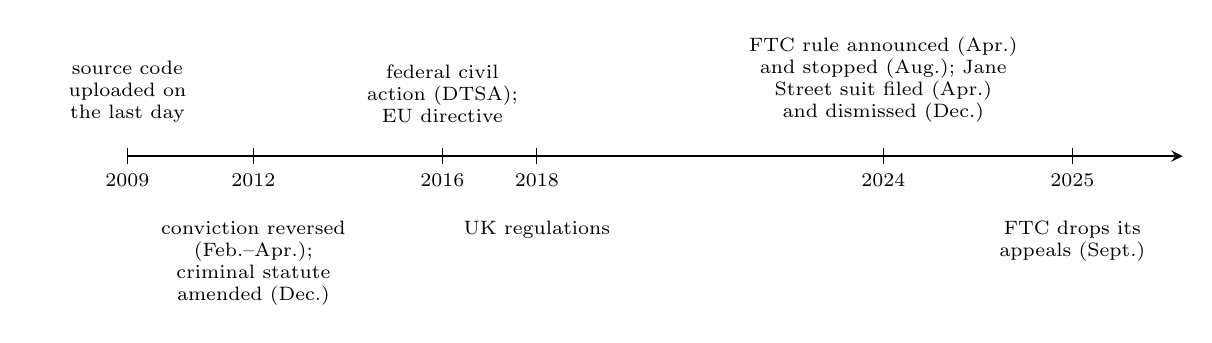
\begin{tikzpicture}[font=\scriptsize,>=stealth]
\draw[->,thick] (0,0) -- (13.4,0);
\foreach \x/\y in {0/2009,1.6/2012,4.0/2016,5.2/2018,9.6/2024,12.0/2025} {\draw (\x,0.1) -- (\x,-0.1) node[below] {\y};}
\node[align=center,anchor=south,text width=2.3cm] at (0,0.3) {source code uploaded on the last day};
\node[align=center,anchor=north,text width=2.6cm] at (1.6,-0.7) {conviction reversed (Feb.--Apr.); criminal statute amended (Dec.)};
\node[align=center,anchor=south,text width=2.3cm] at (4.0,0.3) {federal civil action (DTSA); EU directive};
\node[align=center,anchor=north,text width=2.0cm] at (5.2,-0.7) {UK regulations};
\node[align=center,anchor=south,text width=3.6cm] at (9.6,0.3) {FTC rule announced (Apr.) and stopped (Aug.); Jane Street suit filed (Apr.) and dismissed (Dec.)};
\node[align=center,anchor=north,text width=2.4cm] at (12.0,-0.7) {FTC drops its appeals (Sept.)};
\end{tikzpicture}

\omcaption{The public record of the chapter: the criminal case of the hook and the amendment that followed, the civil statutes, the rise and fall of
the federal non-compete rule, and a civil dispute that ended without a judgement. Sources: the chapter's ledger.}\label{fig:fm:intellectual-property-and-non-competes:record}
\end{omfigure}

\begin{method}[Protecting what leaves with people]\label{met:fm:intellectual-property-and-non-competes:protect}
\begin{enumerate}
\item List what the firm owns in the three kinds (structure, parameters, data) and estimate how fast each loses value once out.
\item Take the reasonable steps: need-to-know access, logged copies and uploads, segregation of duties, confidentiality and invention
assignment in every contract.
\item Set notice and restriction lengths by kind of knowledge (\cref{prop:fm:intellectual-property-and-non-competes:six}), within what local law
allows, and pay for them.
\item At every departure: cut access on resignation, review the logs, remind the employee of the obligations in writing.
\item Take legal advice before relying on any restriction or bringing any claim.
\end{enumerate}
\end{method}

\section{Build: the garden-leave calculator}\label{bld:fm:intellectual-property-and-non-competes:gardenleave}

\begin{build}
\bfield{Purpose} No honest build: the chapter's subject is legal. The analytical tool prices a restriction as a decaying asset against its salary
cost.
\bfield{Interface} \texttt{firm.gardenleave}: \texttt{loss\_if\_start}, \texttt{protected}, \texttt{leave\_cost}, \texttt{net}, \texttt{best\_length},
\texttt{half\_life\_from\_series} (wrapping \texttt{firm.decay.half\_life\_fit}).
\bfield{Rules} Protected value plus remaining loss equals the loss with no restriction; the best length maximises the net value and does not depend
on the discount rate; no restriction is worth it when $LP\le S$.
\bfield{Acceptance tests} \texttt{code/firm/gardenleave/tests/}: the identity, the best length against a grid search, and the half-life of a clean
decay.
\bfield{Stretch} A competitor that needs time to rebuild; a probability that the restriction is not enforced; the expected cost of a leak against
the cost of enforcing a claim.
\end{build}

\begin{omsources}
\item United States v. Aleynikov, 676 F.3d 71 (2d Cir. 2012); Theft of Trade Secrets Clarification Act of 2012, Pub.~L.~112-236.
\item 18 U.S.C. 1836 and 1839; Directive (EU) 2016/943; The Trade Secrets (Enforcement, etc.) Regulations 2018 (SI 2018/597).
\item Federal Trade Commission, Noncompete Rule page and press release of September 2025.
\item Jane Street Group, LLC v. Millennium Management LLC et al., No.~1:24-cv-02783 (S.D.N.Y.), complaint and stipulation of dismissal.
\end{omsources}

\section{Exercises}

\begin{exercise}[$\star$]\label{exo:fm:intellectual-property-and-non-competes:1}
In \cref{ex:fm:intellectual-property-and-non-competes:hand}, compute the value protected by six and twelve months of leave and the loss with no
leave.
\end{exercise}

\begin{exercise}[$\star$]\label{exo:fm:intellectual-property-and-non-competes:2}
List the three conditions for information to be a \omterm{def:fm:intellectual-property-and-non-competes:secret}{trade secret}. Is a signal described in a published paper a \omterm{def:fm:intellectual-property-and-non-competes:secret}{trade secret}? Is the firm's fitted
version of it?
\end{exercise}

\begin{exercise}[$\star$]\label{exo:fm:intellectual-property-and-non-competes:3}
What does \omterm{def:fm:intellectual-property-and-non-competes:restrict}{garden leave} cost for three, six and twelve months at \$1.5 million a year, discounted at 8\%?
\end{exercise}

\begin{exercise}[$\star\star$]\label{exo:fm:intellectual-property-and-non-competes:4}
For which half-life is six months the best length when $LP/S=8$? When $LP/S=4$?
\end{exercise}

\begin{exercise}[$\star\star$]\label{exo:fm:intellectual-property-and-non-competes:5}
Why was the conviction of the hook reversed, and what did Congress change in 2012?
\end{exercise}

\begin{exercise}[$\star\star$]\label{exo:fm:intellectual-property-and-non-competes:6}
Derive the net value at the best length with $r=0$ and check it on \cref{ex:fm:intellectual-property-and-non-competes:hand}.
\end{exercise}

\begin{exercise}[$\star\star\star$]\label{exo:fm:intellectual-property-and-non-competes:7}
\emph{Coding.} Rerun \texttt{fm\_ip.table(seed=12)}. What happens to the half-lives and the best lengths?
\end{exercise}

\begin{exercise}[$\star\star\star$]\label{exo:fm:intellectual-property-and-non-competes:8}
\emph{Find the flaw.} ``Our model's structure is the valuable part. A two-year non-compete protects it fully.''
\end{exercise}

\section{Problem: The Six-Month Question}

\begin{problem}[{Weekend problem --- the six-month question}]\label{pb:fm:intellectual-property-and-non-competes:1}
A senior researcher on a strategy earning \$20 million a year resigns to join a competitor. The head of desk must decide what to protect and
how long to keep the researcher out of the market.

\medskip\noindent\textbf{Part I --- What the firm owns.}
\begin{enumerate}
\item List what a trading firm owns that a competitor cannot buy.
\item Why do patents and copyright protect little of it?
\item Define a \omterm{def:fm:intellectual-property-and-non-competes:secret}{trade secret} and name the condition the firm controls.
\item Define a \omterm{def:fm:intellectual-property-and-non-competes:nda}{confidentiality agreement} and an \omterm{def:fm:intellectual-property-and-non-competes:nda}{invention assignment clause}.
\end{enumerate}

\medskip\noindent\textbf{Part II --- The law.}
\begin{enumerate}[resume]
\item Summarise the facts and the outcome of United States v. Aleynikov.
\item What did the 2012 amendment change, and what did the 2016 Act add?
\item What is the status of the FTC's non-compete rule?
\item What did the Jane Street complaint allege, and how did the case end?
\end{enumerate}

\medskip\noindent\textbf{Part III --- The model.}
\begin{enumerate}[resume]
\item Define a \omterm{def:fm:intellectual-property-and-non-competes:restrict}{non-compete clause}, \omterm{def:fm:intellectual-property-and-non-competes:restrict}{garden leave} and a \omterm{def:fm:intellectual-property-and-non-competes:restrict}{non-solicitation clause}.
\item Write the protected value and the cost of a restriction of length $T$.
\item State and prove \cref{prop:fm:intellectual-property-and-non-competes:six}.
\item Give the fitted half-lives of the three kinds of knowledge.
\item Give the value protected by six months for each, and its share of the loss with no leave.
\item Give the best lengths, and say why each is that many half-lives.
\end{enumerate}

\medskip\noindent\textbf{Part IV --- The decision.}
\begin{enumerate}[resume]
\item The researcher knows the structure and the parameters. How long a restriction would you want, and what does six months buy?
\item What protects the structure beyond any restriction?
\item List the steps to take on the day of the resignation.
\item How robust are the best lengths to the noise in the half-life estimates?
\item State the \emph{named result}: the garden-leave length at which the marginal edge protected equals the marginal salary cost.
\item In two sentences, write the firm's policy on restrictions.
\end{enumerate}
\end{problem}

\section{Interview questions}

\begin{interviewq}[$\star$ \iqroles{researcher, trader}]\label{iq:fm:intellectual-property-and-non-competes:1}
What is \omterm{def:fm:intellectual-property-and-non-competes:restrict}{garden leave}, and why would a firm pay you not to work?
\end{interviewq}

\begin{interviewq}[$\star$ \iqroles{developer}]\label{iq:fm:intellectual-property-and-non-competes:2}
You wrote a backtesting library at your last job. Can you bring it with you?
\end{interviewq}

\begin{interviewq}[$\star\star$ \iqroles{researcher}]\label{iq:fm:intellectual-property-and-non-competes:3}
A signal's value halves every six months. How much of it does a six-month non-compete protect?
\end{interviewq}

\begin{interviewq}[$\star\star$ \iqroles{risk}]\label{iq:fm:intellectual-property-and-non-competes:4}
What would you log to show that the firm takes reasonable steps to keep its code secret?
\end{interviewq}

\begin{interviewq}[$\star\star$ \iqroles{researcher}]\label{iq:fm:intellectual-property-and-non-competes:5}
Which leaks faster in value: a model's parameters or its structure? What follows for a firm's contracts?
\end{interviewq}

\begin{interviewq}[$\star\star\star$ \iqroles{researcher, trader}]\label{iq:fm:intellectual-property-and-non-competes:6}
Derive the length of \omterm{def:fm:intellectual-property-and-non-competes:restrict}{garden leave} that maximises its net value to the firm.
\end{interviewq}
